\documentclass{article}\usepackage[]{graphicx}\usepackage[]{color}
%% maxwidth is the original width if it is less than linewidth
%% otherwise use linewidth (to make sure the graphics do not exceed the margin)
\makeatletter
\def\maxwidth{ %
  \ifdim\Gin@nat@width>\linewidth
    \linewidth
  \else
    \Gin@nat@width
  \fi
}
\makeatother

\definecolor{fgcolor}{rgb}{0.345, 0.345, 0.345}
\newcommand{\hlnum}[1]{\textcolor[rgb]{0.686,0.059,0.569}{#1}}%
\newcommand{\hlstr}[1]{\textcolor[rgb]{0.192,0.494,0.8}{#1}}%
\newcommand{\hlcom}[1]{\textcolor[rgb]{0.678,0.584,0.686}{\textit{#1}}}%
\newcommand{\hlopt}[1]{\textcolor[rgb]{0,0,0}{#1}}%
\newcommand{\hlstd}[1]{\textcolor[rgb]{0.345,0.345,0.345}{#1}}%
\newcommand{\hlkwa}[1]{\textcolor[rgb]{0.161,0.373,0.58}{\textbf{#1}}}%
\newcommand{\hlkwb}[1]{\textcolor[rgb]{0.69,0.353,0.396}{#1}}%
\newcommand{\hlkwc}[1]{\textcolor[rgb]{0.333,0.667,0.333}{#1}}%
\newcommand{\hlkwd}[1]{\textcolor[rgb]{0.737,0.353,0.396}{\textbf{#1}}}%

\usepackage{framed}
\makeatletter
\newenvironment{kframe}{%
 \def\at@end@of@kframe{}%
 \ifinner\ifhmode%
  \def\at@end@of@kframe{\end{minipage}}%
  \begin{minipage}{\columnwidth}%
 \fi\fi%
 \def\FrameCommand##1{\hskip\@totalleftmargin \hskip-\fboxsep
 \colorbox{shadecolor}{##1}\hskip-\fboxsep
     % There is no \\@totalrightmargin, so:
     \hskip-\linewidth \hskip-\@totalleftmargin \hskip\columnwidth}%
 \MakeFramed {\advance\hsize-\width
   \@totalleftmargin\z@ \linewidth\hsize
   \@setminipage}}%
 {\par\unskip\endMakeFramed%
 \at@end@of@kframe}
\makeatother

\definecolor{shadecolor}{rgb}{.97, .97, .97}
\definecolor{messagecolor}{rgb}{0, 0, 0}
\definecolor{warningcolor}{rgb}{1, 0, 1}
\definecolor{errorcolor}{rgb}{1, 0, 0}
\newenvironment{knitrout}{}{} % an empty environment to be redefined in TeX

\usepackage{alltt}
\usepackage[total={3in, 8in}]{geometry}
\usepackage{graphicx}
\usepackage{color}
\usepackage{bold-extra}
\pagestyle{empty}
\def\tilde{\texttt{\~}}
\newcommand{\Wspace}{{\tiny\color{white}.}\hfill}
\newcommand{\NewSection}[1]{{\noindent\color{blue}\bfseries\scshape#1}}



%\AtBeginDocument{\raggedright}
\IfFileExists{upquote.sty}{\usepackage{upquote}}{}
\begin{document}
\NewSection{Load Packages}\hfill\verb+require(mosaic)+\\ 
\hspace*{1cm}\hfill\verb+require(mosaicData)+\\
\\
\NewSection{Essential R Syntax}\\
Function \& arguments:\hfill \verb+rflip(10)+\\
Optional arguments:\hfill \verb+rflip(10, prob=0.3)+\\
Assignment:\hfill \verb+x <- rflip(10, prob=0.3)+\\
\\
\NewSection{Formula Interface}\\
Used for graphics, statistics, inference, and modeling operations.\\
\def\phbox#1{\fbox{\phantom{g#1l}}} %
\def\ffbox#1{\fbox{\phantom{g}#1\phantom{b}}} %
\vspace*{-.5cm}\begin{center}
	\sf
	\ffbox{goal} $\Big($ 
	\ffbox{y} $\sim$  \ffbox{x} {\LARGE,} data = \ffbox{mydata} $\Big)$
\end{center}
\noindent {\small Read as:} {Calculate {\sf goal} using {\sf mydata} for {\sf y} ``broken down" by {\sf x}, or ``modeled by" {\sf x}.} Examples:\\
\Wspace\verb+mean(age~homeless, data=HELPrct)+%
\vspace*{-2mm}
\begin{knitrout}
\definecolor{shadecolor}{rgb}{0.816, 0.816, 0.941}\color{fgcolor}\begin{kframe}
\begin{verbatim}
|  homeless   housed 
|      36.4     35.0
\end{verbatim}
\end{kframe}
\end{knitrout}
\noindent\Wspace\verb+quantile(age~sex,data=HELPrct,p=c(.2,.8))+%
\vspace*{-6mm}
\begin{knitrout}
\definecolor{shadecolor}{rgb}{0.816, 0.816, 0.941}\color{fgcolor}\begin{kframe}
\begin{verbatim}
|    .group 20%  80%
|  1 female  30 42.8
|  2   male  29 41.0
\end{verbatim}
\end{kframe}
\end{knitrout}
\Wspace\verb+tally(homeless~sex, data=HELPrct)+%
\vspace*{-2mm}
\begin{knitrout}
\definecolor{shadecolor}{rgb}{0.816, 0.816, 0.941}\color{fgcolor}\begin{kframe}
\begin{verbatim}
|            sex
|  homeless   female  male
|    homeless  0.374 0.488
|    housed    0.626 0.512
\end{verbatim}
\end{kframe}
\end{knitrout}
\NewSection{RMarkdown documents}\\
\\
\hbox{\fbox{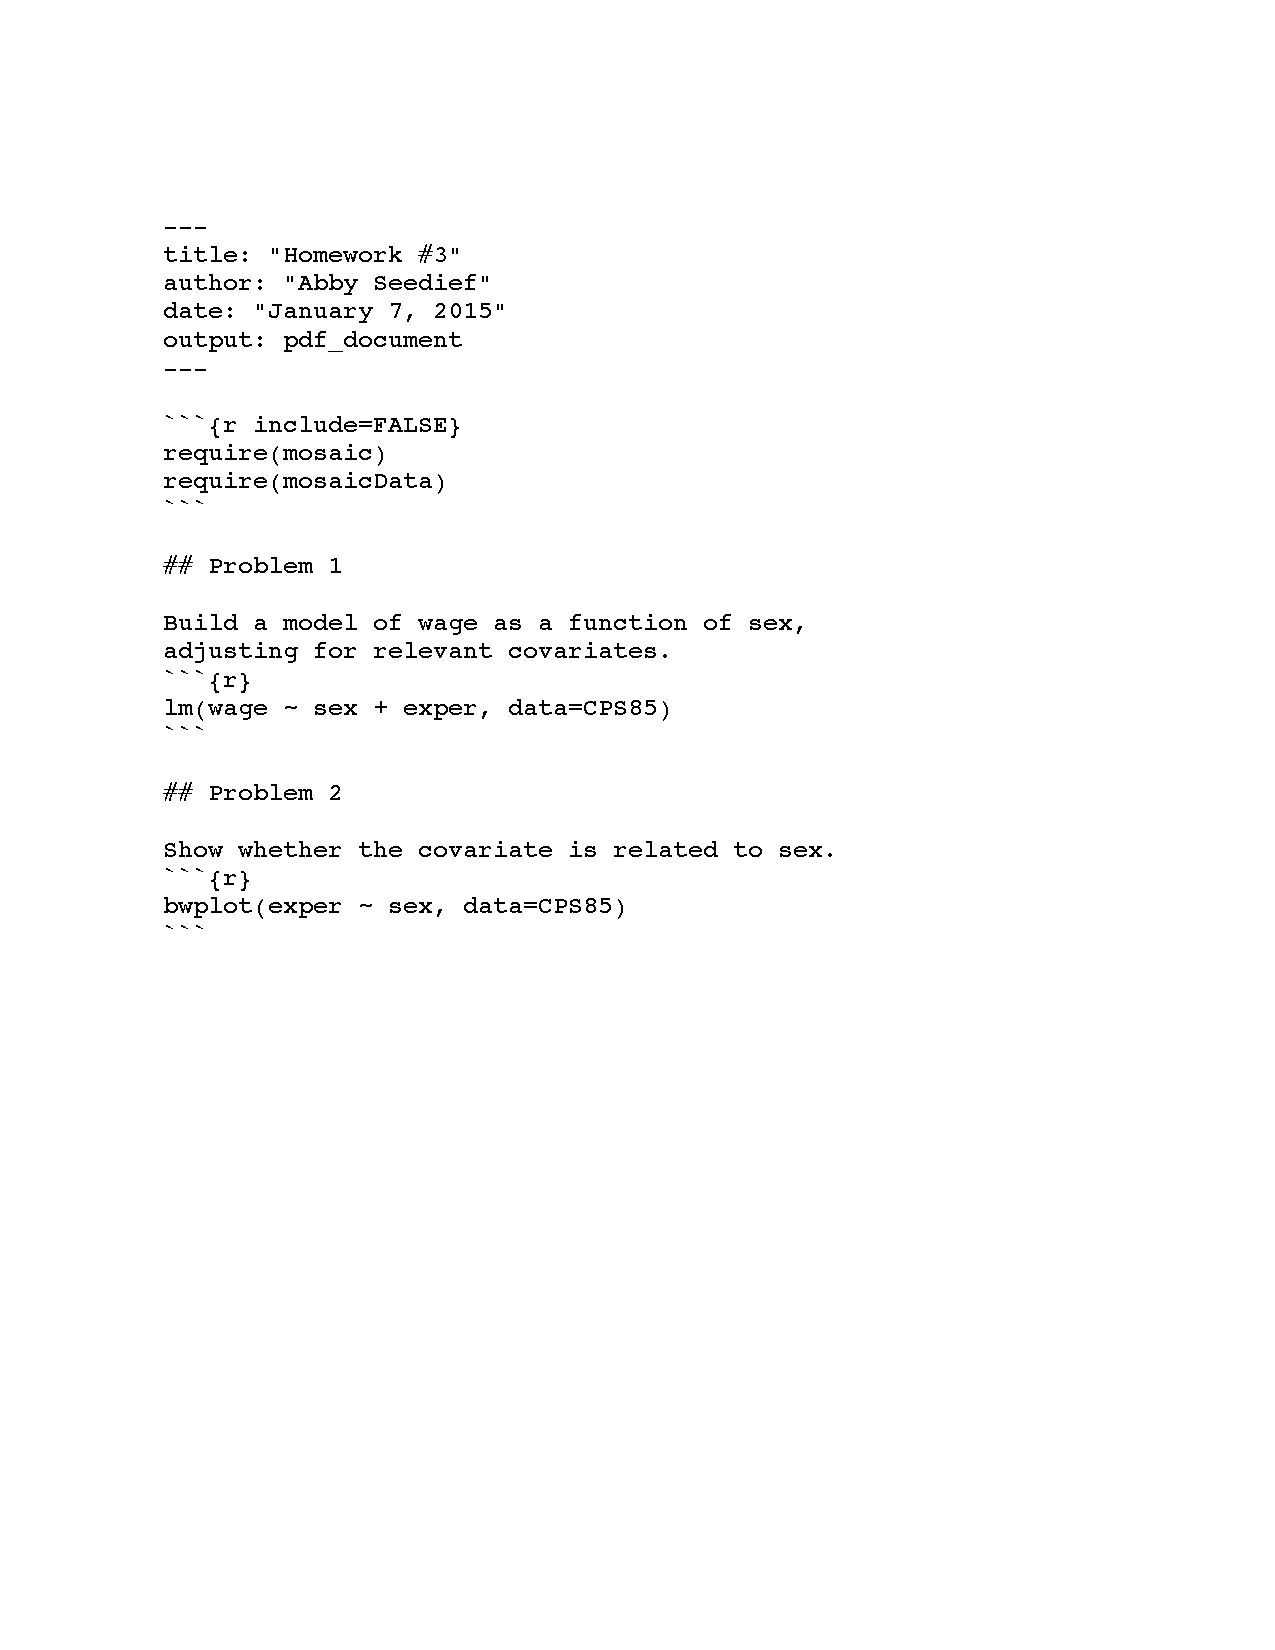
\includegraphics[width=1.6in]{RMarkdown-example-source.pdf}} \hfill \fbox{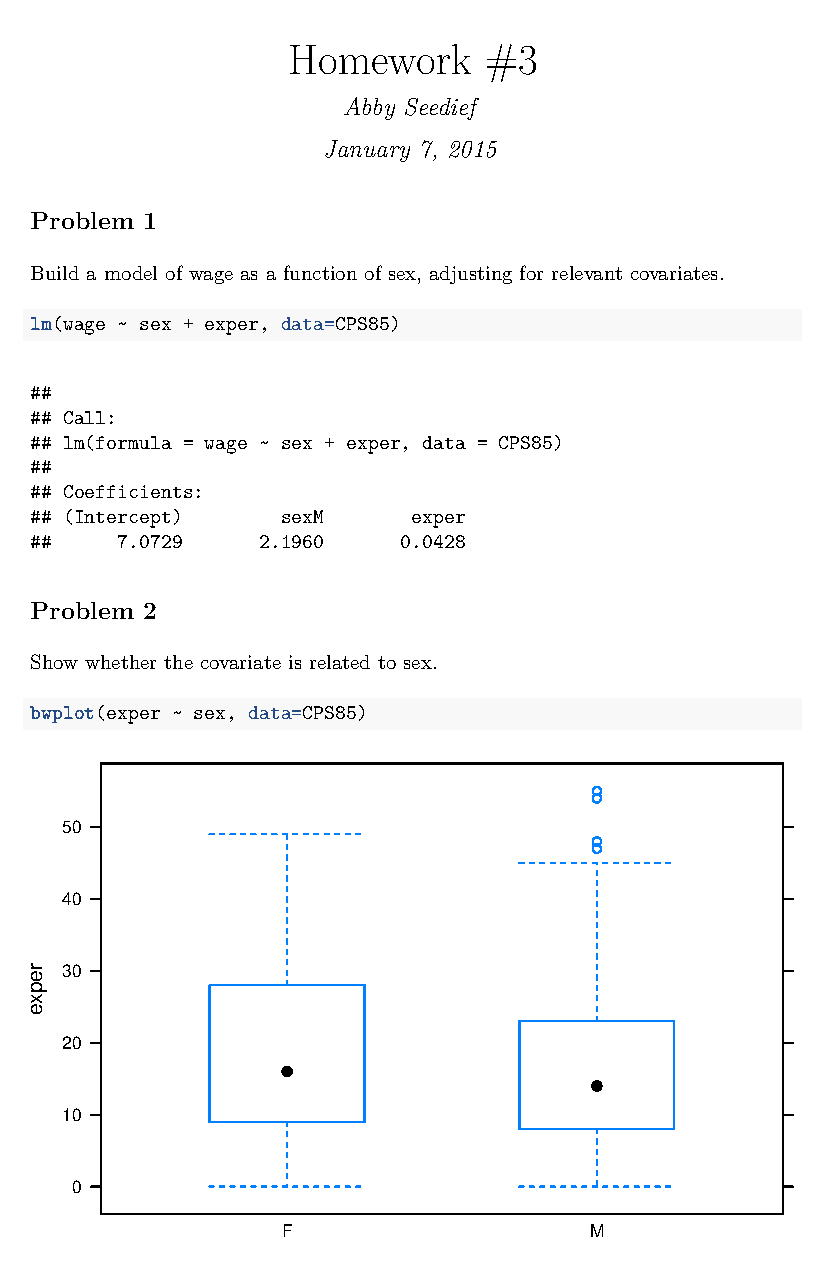
\includegraphics[width=1.2in]{RMarkdown-example.pdf}}}\\
\begin{small}%
\noindent Compile to any of HTML, PDF, or Word.\\
See \texttt{mosaic plain} template through RStudio menu:\\ 
{\sc File/New File/RMarkdown/From Template}
\end{small}%

\newpage
\hrule\vspace*{1mm}%
\NewSection{Graphics Formula Syntax}\\
\noindent{\sf
	\ffbox{goal} $\Big($ 
	\ffbox{y} $\sim$  \ffbox{x} {$\ \Big\boldmath|\ $} \ffbox{z} {\LARGE,}}\\\Wspace 
  {\sf groups=\ffbox{w} , data = \ffbox{mydata} $\Big)$}


\noindent$\bullet$ {\sf y} --- y-axis variable ({\sc optional})\\
$\bullet$ {\sf x} --- x-axis variable ({\sc\color{blue}Required})\\
$\bullet$ {\sf z} --- facet-by variable ({\sc optional})\\
$\bullet$ {\sf w} --- color-by variable ({\sc optional})\\
\vspace*{-2mm}
\hrule
\noindent%
\hspace*{-2mm}%
\begin{knitrout}
\definecolor{shadecolor}{rgb}{0.816, 0.816, 0.941}\color{fgcolor}
\includegraphics[width=1in,height=2cm]{figure/unnamed-chunk-5-1} 
\includegraphics[width=1in,height=2cm]{figure/unnamed-chunk-5-2} 
\includegraphics[width=1in,height=2cm]{figure/unnamed-chunk-5-3} 

\end{knitrout}
\begin{small}
\noindent {\tiny \sc Left:}\hfill\verb+bwplot(wage~sex, data= CPS85)+\\
{\tiny \sc Middle:}\hfill\verb+xyplot(wage~educ | sex, data= CPS85)+\\
{\tiny \sc Right:}\hfill\verb+xyplot(wage~educ, groups=sex, data=CPS85)+\\
\end{small}
\hrule%
\noindent\hspace*{-2mm}%
\begin{knitrout}
\definecolor{shadecolor}{rgb}{0.816, 0.816, 0.941}\color{fgcolor}
\includegraphics[width=1in,height=2cm]{figure/unnamed-chunk-6-1} 
\includegraphics[width=1in,height=2cm]{figure/unnamed-chunk-6-2} 
\includegraphics[width=1in,height=2cm]{figure/unnamed-chunk-6-3} 

\end{knitrout}
\begin{small}
\noindent {\tiny \sc Left:}\hfill\verb+densityplot(~wage, data= CPS85)+\\
{\tiny \sc Middle:}\hfill\verb+densityplot(~wage | sex, data= CPS85)+\\
{\tiny \sc Right:}\hfill\verb+densityplot(~wage,groups=sex, data=CPS85)+\\
\end{small}
\hrule
\hrule
\vspace*{2mm}
\NewSection{Randomization and Iteration}\\
\begin{small}
\noindent{\sc Resample/Bootstrap:}\\
\verb+do(100)*mean(wage ~ sex, data=resample(CPS85))+\\
{\sc Random Permutations:}\\
\verb+do(100)*mean(wage ~ shuffle(sex), data=CPS85)+\\
\end{small}
\hrule
\hrule
\vspace*{2mm}
\NewSection{Confidence Intervals \& Statistical Tests}\\
\begin{small}\Wspace\verb+t.test(wage ~ sex, data=CPS85)+\\
\Wspace\verb+prop.test(43, 100)+\\
\Wspace\verb#crosstab <- tally(~union+sex, data=CPS85)#\\
\Wspace\verb#chisq.test( crosstab )  fisher.test(crosstab)#\\
\Wspace\verb+mod <- lm(wage ~ sector, data=CPS85)+\\
\Wspace{Then ... \verb+anova(mod)    TukeyHSD(mod)+   etc.}\\
\noindent{\bf\sc\small Modeling \& Covariates}\\
\Wspace\verb#mod <- lm(wage ~ sex + educ, data=CPS85)#\\
\Wspace\verb#summary(mod)# or \verb#anova(mod)# or \verb#confint(mod)#\\
\noindent {\sc\small Extract model function:}\\
\Wspace\verb+fun <- makeFun(mod)+\\
\Wspace \verb+fun(sex="F",educ=10)+}\\
\Wspace{\footnotesize{\small\verb+plotFun(+}\verb+fun(sex="F",educ=x)} ~ x,x.lim=range(0,8))+}\\\hrule
\end{small}
\vfill

\end{document}
